\documentclass[12pt]{article}
\usepackage[utf8]{inputenc}
\usepackage{amsmath}
\usepackage{mathtools}
\usepackage{amsfonts}
\usepackage{lastpage}
\usepackage{tikz}
\usepackage{pdfpages}
\usepackage{gauss}
\usepackage{fancyvrb}
\usepackage{fancyhdr}
\usepackage{graphicx}
\pagestyle{fancy}
\fancyfoot[C]{\footnotesize Page \thepage\ of 3}
\DeclareGraphicsExtensions{.pdf,.png,.jpg}
\title{Lynopgave 1}
\author{Nikolaj Dybdahl Rathcke and Victor Petren Bach Hansen}
\chead{Nikolaj Dybdahl Rathcke (rfq695) - Victor Petren Bach Hansen (grn762)}

\begin{document}
\section*{MatIntroNat - Lynopgave 3}
\subsection*{Opgave 9.1}
Tegn en skitse af mængden
$$D= \{(x,y)\:|\: 0\leq y\leq 2, 1-y\leq x\leq 1\}$$
Udregn planintegralet af $x^2y$ over $D$ som et itereret integral med integrationen m.h.t $x$ inderst.\\
Opskriv dernæst den samme mængde $D$ på lærebogens form og udregn det samme planintegral, nu med integrationen m.h.t $x$ yderst.\\
Illustrer ved brug af Maple den figur, hvis rumfang integralet udtrykker.\\
\\
Vi starter med at skitsere mængden $D$ ved brug af Maple\\
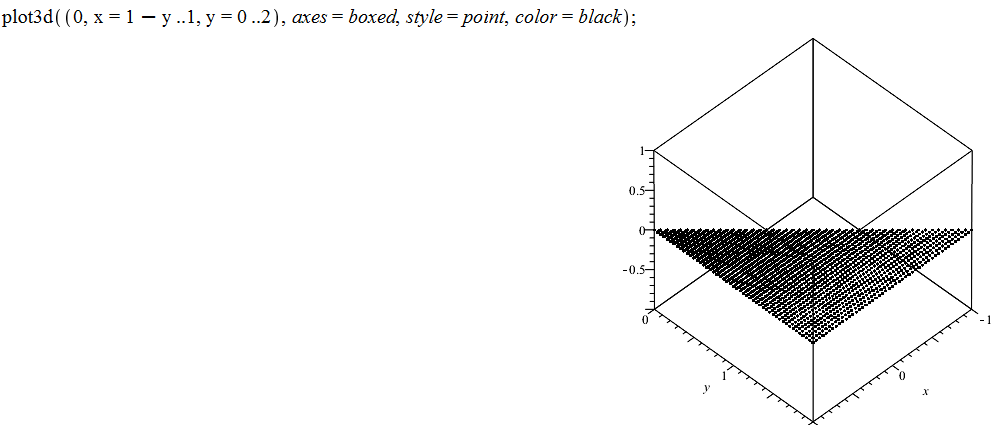
\includegraphics[scale=0.6]{Pic1}\\
Herefter beregner vi planintegralet af $x^2y$ over $D$ på formen (\textbf{5.2}) m.h.t $x$ inderst\\
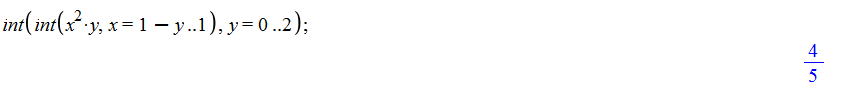
\includegraphics[scale=0.6]{Pic2}\\
Derefter beregnes planintegralet af $x^2y$ over $D$ på formen (\textbf{5.1}) m.h.t $x$ yderst\\
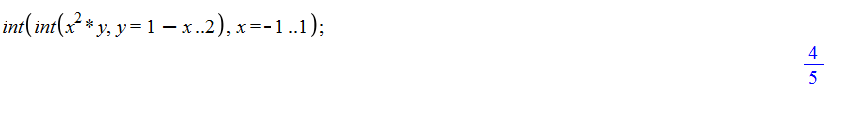
\includegraphics[scale=0.6]{Pic3}\\
Nedenfor er figuren, hvis rumfang integralet udtrykker vist\\
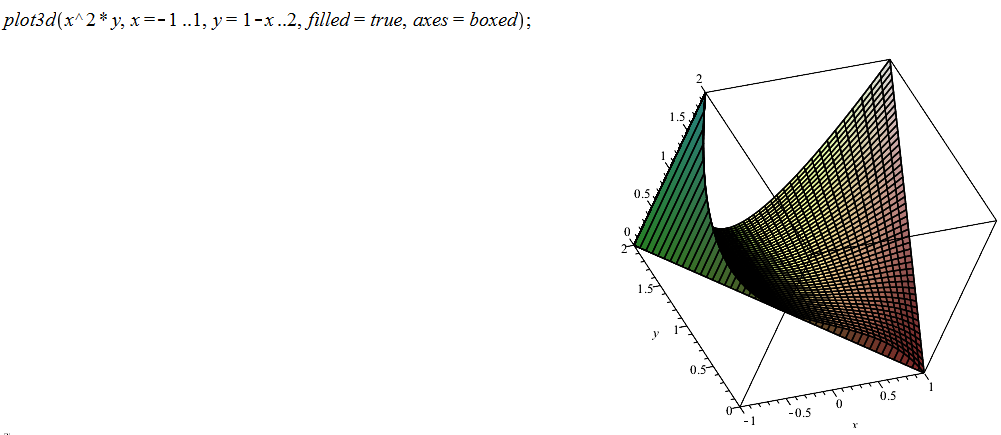
\includegraphics[scale=0.6]{Pic4}\\
Det er ligemeget hvilken form af $D$ vi bruger, ovenfor er brugt den der er skrevet på (\textbf{5.1}).

\newpage
\subsection*{Opgave 9.3}
Udtryk mængden
$$R=\{(x,y,z)\:|\: 0\leq y, x^2+y^2+z^2\leq 1\}$$
i sfæriske koordinater, og udregn derefter rumintegralet af funktionen $f(x,y,z)=y$ over $R$.\\
\\
Vi udtrykker mængden $R$ med sfæriske koordinater
\begin{align*}
x&=\rho cos(\theta)sin(\phi)\\
y&=\rho sin(\theta)sin(\phi)\\
z&=\rho cos(\phi)
\end{align*}

Hvor vi så kan skrive betingelserne for mængden $R$ som
$$0\leq \rho sin(\theta)sin(\phi)$$
og
$$(\rho cos(\theta)sin(\phi))^2+(\rho sin(\theta)sin(\phi))^2+(\rho cos(\phi))^2\leq1$$
$$\rho^2((cos(\theta)^2+sin(\theta)^2)sin(\phi)^2+cos(\phi)^2\leq1$$
$$\rho^2(sin(\phi)^2+cos(\phi)^2\leq1$$
$$\rho^2\leq1$$
Så vi har nu mængden $R$ udtryk i sfæriske koordinater ved
$$R=\{(\rho,\theta,\phi)\:|\: 0\leq \rho sin(\theta)sin(\phi),\rho^2\leq 1\}$$
Altså er mængden $R$ er lukket og begrænset og er en halvkugle, da $0\leq y$, med en radius på $1$ da $\rho^2\leq1$.\\
Vi omskriver derfor mængden $R$
$$R=\{(\rho,\theta,\phi)\:|\: 0\leq\rho\leq 1,0\leq\theta\leq \pi, 0\leq\phi\leq\pi\}$$
Her er $\theta$ begrænset til $0\leq\theta\leq\pi$ da der er tale om en halvkuglen.\\
Rumintegralet af funktionen $f(x,y,z)=y$ over $R$ er således\\
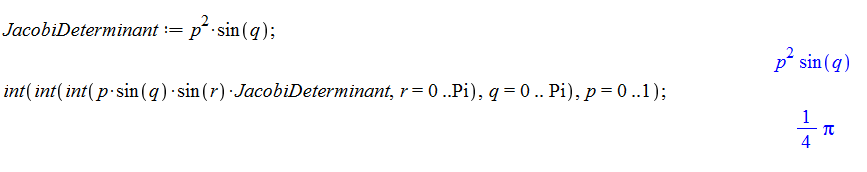
\includegraphics[scale=0.6]{Pic5}\\
hvor $p=\rho,q=\theta$ og $r=\phi$.



\end{document}



